
\begin{table*}[t!]
    \centering
    % 第一个表格
    \begin{minipage}{0.25\textwidth}
        \centering
        \resizebox{\textwidth}{!}{
        \begin{tabular}{c|c|c|c|c}
        \toprule
        \ &
          \multicolumn{1}{c|}{FID$\downarrow$} &
          \multicolumn{1}{c|}{FVD$\downarrow$} &
          \multicolumn{1}{c|}{Sync-C$\uparrow$} &
          \multicolumn{1}{c}{Sync-D$\downarrow$} \\ 
          \midrule
        SadTalker~\cite{zhang2022sadtalker}   & 22.340 & 203.860 & \textbf{7.885} & \textbf{7.545}  \\
        DreamTalk~\cite{ma2023dreamtalk}      & 78.147 & 790.660 & 6.376 & 8.364  \\
        AniPortrait~\cite{wei2024aniportrait} & 26.561 & 234.666 & 4.015 & 10.548  \\
        Hallo~\cite{xu2024hallo}              & 20.545 & 173.497 & 7.750 & 7.659  \\
        Ours                                  & \textbf{20.359} & \textbf{160.838} & 7.252 & 8.106  \\ 
        \midrule
        Real video                            & - & - & 8.700 & 6.597 \\ 
        \bottomrule
        \end{tabular}}
        \vspace{-2mm}
        \caption{Comparison with the other methods on HDTF dataset.} 
        \label{tab:comp_hdtf}
    \end{minipage}
    \hfill
    % 第二个表格
    \begin{minipage}{0.30\textwidth}
        \centering
        \resizebox{\textwidth}{!}{
        \begin{tabular}{c|c|c|c|c|c}
        \toprule
            \ &
              \multicolumn{1}{c|}{FID$\downarrow$} &
              \multicolumn{1}{c|}{FVD$\downarrow$} &
              \multicolumn{1}{c|}{Sync-C$\uparrow$} &
              \multicolumn{1}{c|}{Sync-D$\downarrow$} &
              \multicolumn{1}{c}{E-FID$\downarrow$} \\ 
              \midrule
            SadTalker~\cite{zhang2022sadtalker}   & 50.015 & 471.163 & 6.922 & \textbf{7.921} & 95.194 \\
            DreamTalk~\cite{ma2023dreamtalk}      & 109.011 & 988.539 & 5.709 & 8.743 & 153.450 \\
            AniPortrait~\cite{wei2024aniportrait} & 46.915 & 477.179 & 2.853 & 11.709 & 88.986 \\
            Hallo~\cite{xu2024hallo}              & 44.578 & 377.117 & \textbf{7.191} & 7.984 & 78.495 \\
            Ours                                  & \textbf{43.271} & \textbf{355.272} & 6.527 & 9.113 & \textbf{71.210} \\ 
            \midrule
            Real video                            & - & - & 7.372 & 7.518 & - \\ 
            \bottomrule
        \end{tabular}}
        \vspace{-2mm}
        \caption{Comparison with other methods on Celeb-V dataset.}
        \label{tab:comp_celebv}
    \end{minipage}
    \hfill
    % 第三个表格
    \begin{minipage}{0.39\textwidth}
        \centering
        \resizebox{\textwidth}{!}{
        \begin{tabular}{c|c|c|c|c|c|c}
        \toprule
        \ &
          \multicolumn{1}{c|}{Sync-C$\uparrow$} &
          \multicolumn{1}{c|}{Sync-D$\downarrow$} &
          \makecell{Subject\\Dynamic$\uparrow$} &
          \makecell{Background\\Dynamic$\uparrow$} &
          \makecell{Subject\\FVD$\downarrow$} &
          \makecell{Background\\FVD$\downarrow$} \\ 
          \midrule   
        SadTalker~\cite{zhang2022sadtalker}  & 3.845           & 10.378         & 2.953   & 0.220 & 470.377 &313.758 \\
        DreamTalk~\cite{ma2023dreamtalk}     & 4.498           & 11.005         & 6.958   & 1.806 & 835.480 &744.177 \\
        AniPortrait~\cite{wei2024aniportrait}&	1.685           & 12.025        & 3.351  & 1.769 & 473.173 & 302.716 \\
        Hallo~\cite{xu2024hallo}             & 4.654           & 10.202         & 5.268   & 1.272 & 394.627 & 291.052 \\
        Ours                                 & \textbf{6.154}  & \textbf{8.574} & 
         \textbf{13.286}  & \textbf{4.481} & \textbf{359.493} &\textbf{248.283} \\ 
        \bottomrule
        \end{tabular}}
        \vspace{-2mm}
        \caption{Comparison with other methods on our proposed wild dataset.}
        \label{tab:comparison_wild}
    \end{minipage}
    \vspace{2mm}
\end{table*}


\begin{figure*}[t!]
    \centering
    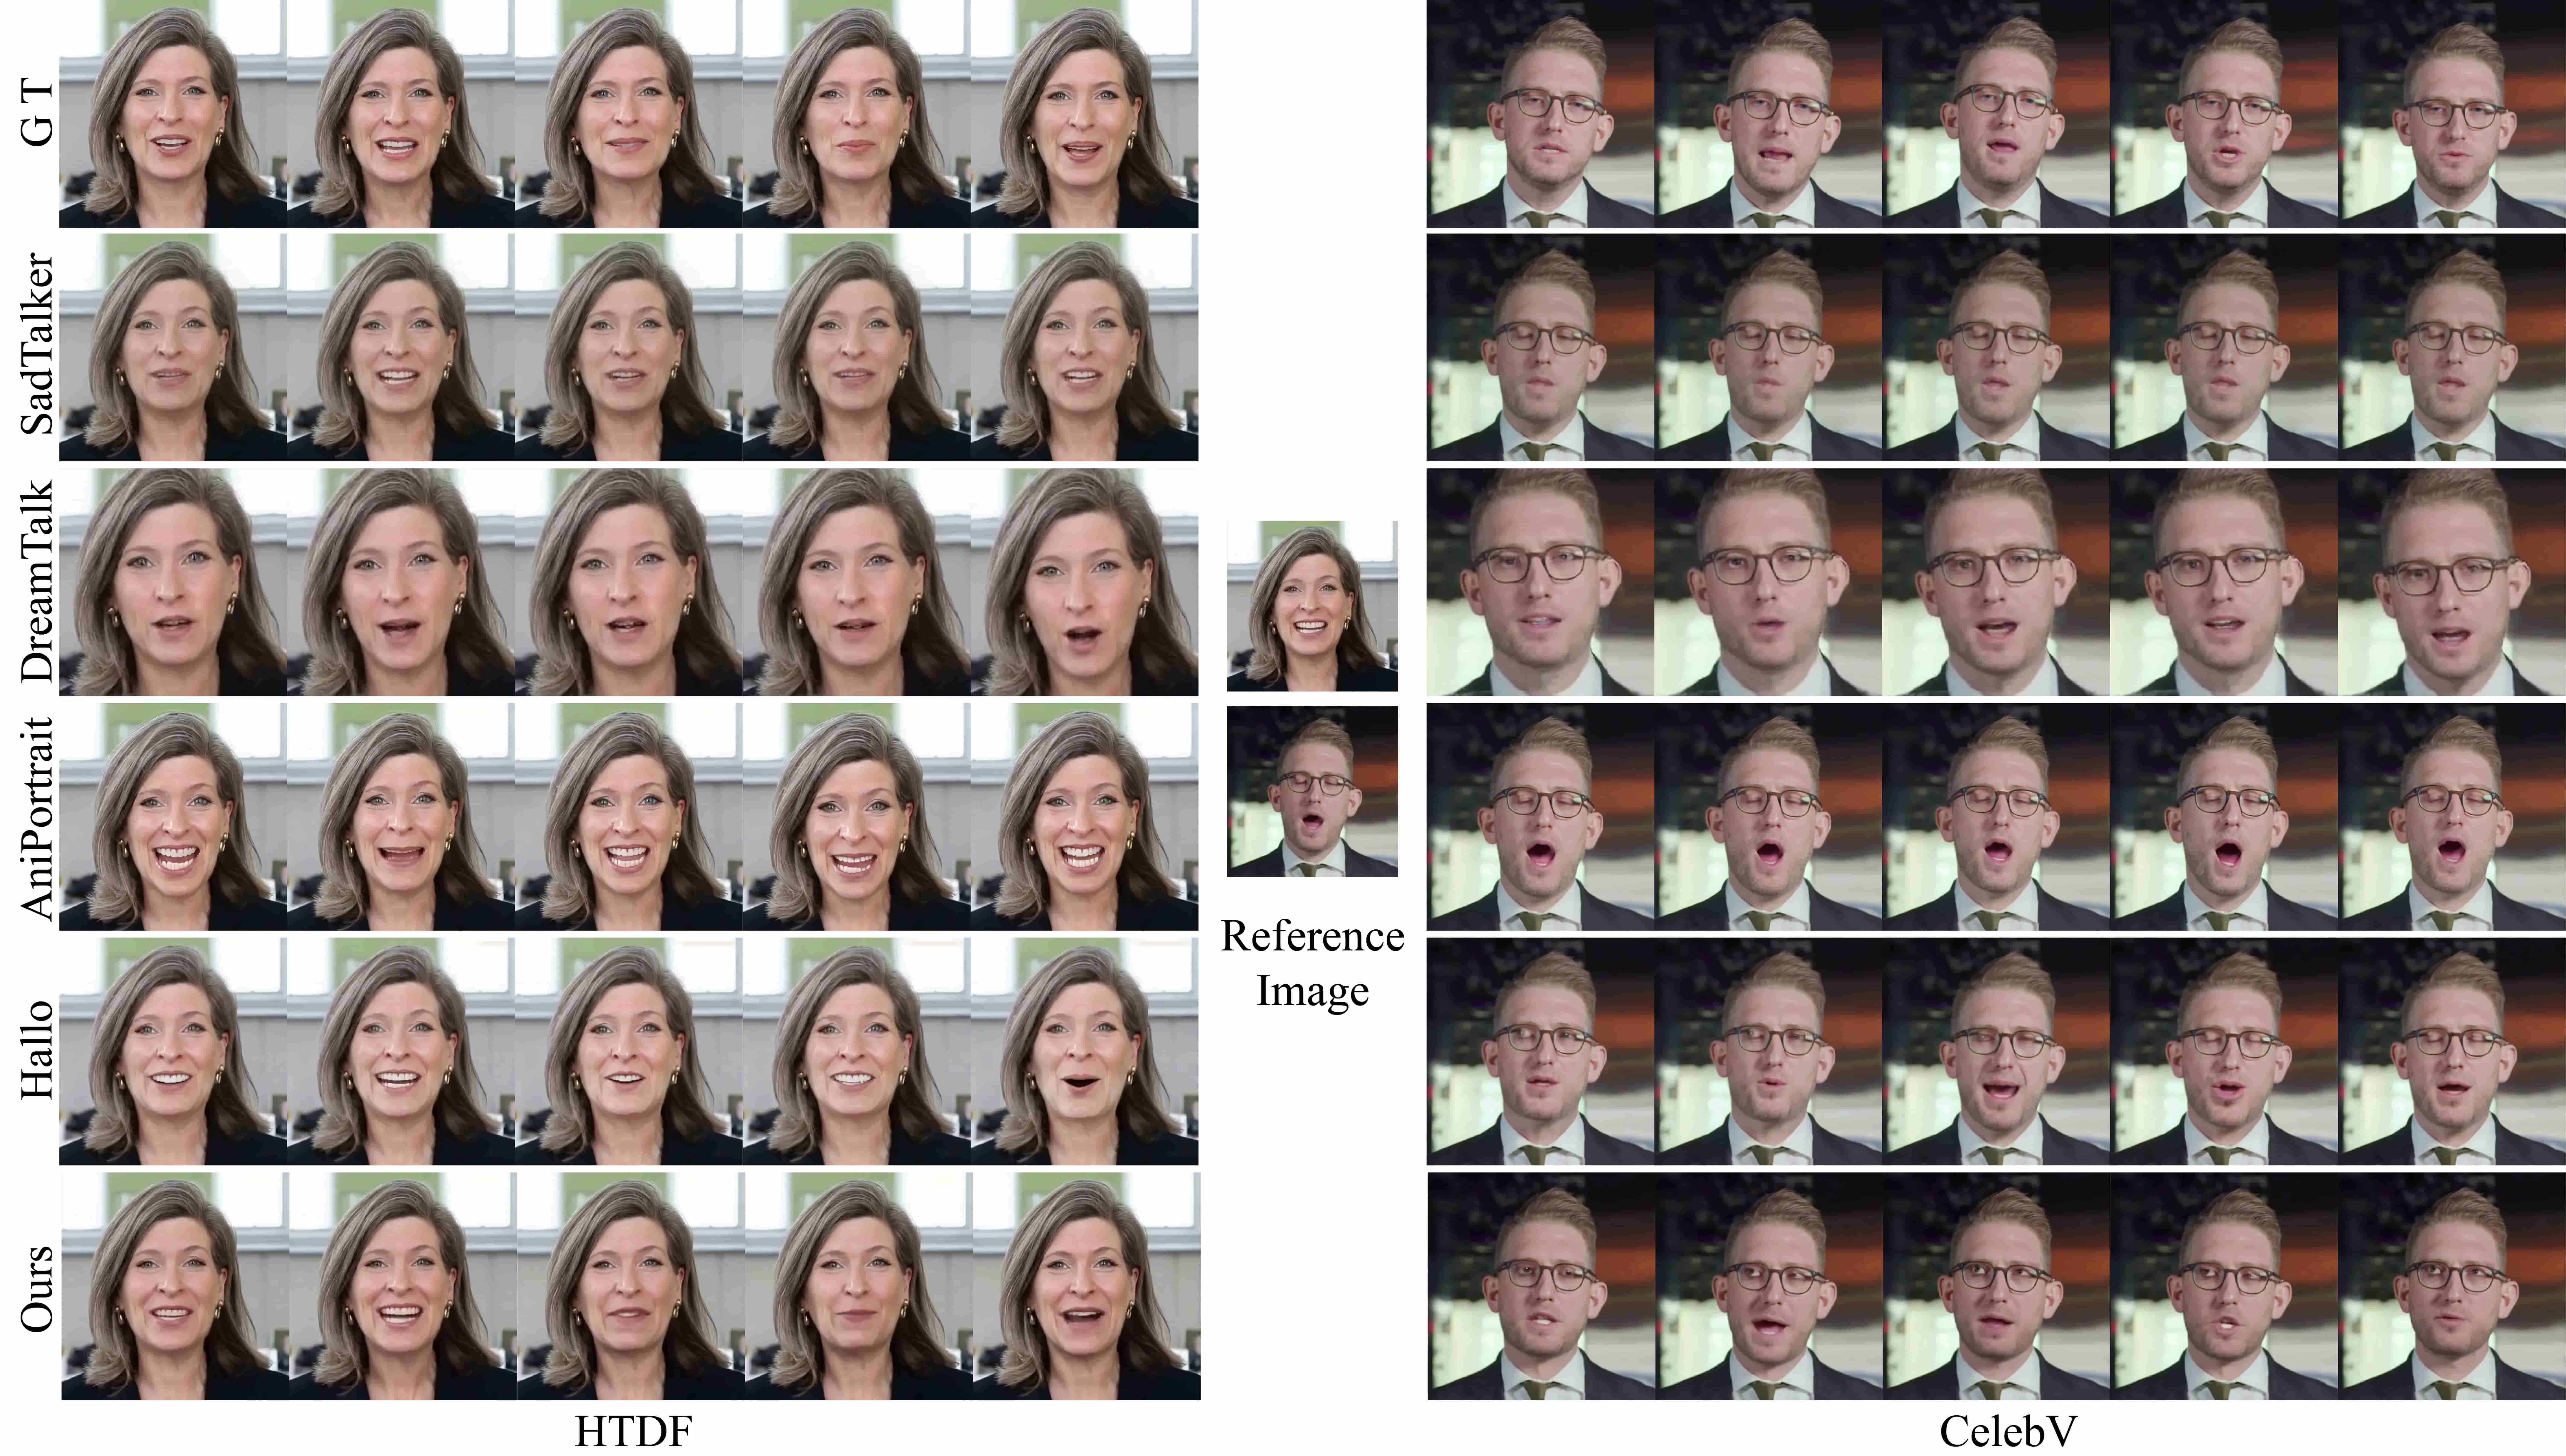
\includegraphics[width=\linewidth]{figs/HTDF_CelebV_comp.jpg}
    \vspace{-6mm}
    \caption{Qualitative comparison on the HTDF~(left) and CelebV~(right) data-set.}
    \vspace{-2mm}
    \label{fig:hdtf}
\end{figure*}





% \begin{figure}[th!]
%     \centering
%     % Creates an empty box with dimensions
%     % \rule{\linewidth}{0.5\linewidth}
%     \includegraphics[width=1\linewidth]{figs/comparisn_of_audio_conditioning2.pdf}
%     \caption{Qualitative comparison of different strategies for audio conditioning.}
%     \label{fig:comparisn_of_audio_conditioning2}
%     \vspace{-4mm}
% \end{figure}

% \begin{figure}[th!]
%     \centering
%     % Creates an empty box with dimensions
%     % \rule{\linewidth}{0.5\linewidth}
%      \includegraphics[width=1\linewidth]{figs/Comparison_of_the_appearance_reference_network.pdf}
%     \caption{ Qualitative comparison of different strategies for indentity conditioning.}
%     \label{fig:Comparison_of_the_appearance_reference_network}
% \end{figure}

\section{Experiment}
\subsection{Experimental Setups}
% \noindent\textbf{Comparison on dynamic scene scenarios.}

\noindent\textbf{Implementation.}
% {The model was trained using 64 NVIDIA A100 GPUs. In addition to training, all experiments were conducted on a GPU server equipped with 8 NVIDIA A100 GPUs. The first and second stages of the model were trained 20,000 steps respectively. During training, the batch size of each GPU was 1, and the learning rate was set to 1e-5. The resolution of the training video is 480 x 720, and it can generate a video with 49 frames at a time. In the training process, the audio embedding is dropped with a probability of 0.05, and the motion frames are randomly masked with a probability of 0.25.}
We initialize the identity reference and denoising networks with weights derived from CogVideoX-5B-I2V\cite{yang2024cogvideox}. During both training phases, we employ the v-prediction diffusion loss\cite{salimans2022progressive} for optimization. Each training phase comprises 20,000 steps, utilizing 64 NVIDIA H100 GPUs. The batch size per GPU is set to 1, with a learning rate of \(480 \times 720\) pixels. To enhance video generation variability, the reference image, guidance audio and textual prompt are dropped with a probability of 0.05 during training.

\noindent\textbf{Evaluation Metrics.}
We employed a range of evaluation metrics for generated videos across benchmark datasets, including HDTF~\cite{zhang2021flow} and Celeb-V~\cite{zhu2022celebvhq}. 
These metrics comprise Fréchet Inception Distance (FID)~\cite{Seitzer2020FID}, Fréchet Video Distance (FVD)~\cite{unterthiner2018towards}, Synchronization-C (Sync-C)~\cite{Chung16a}, Synchronization-D (Sync-D)~\cite{Chung16a}, and E-FID~\cite{tian2024emo}. 
FID and FVD quantify the similarity between generated images and real data, while Sync-C and Sync-D assess lip synchronization accuracy. E-FID evaluates the image quality based on features extracted from the Inception network.
Besides, we introduced VBench~\cite{huang2023vbench} metrics to enhance evaluation, focusing on dynamic degree and subject consistency. 
% Background consistency is evaluated via CLIP feature similarity, assessing the temporal stability of backgrounds. 
%Temporal flickering is quantified by mean absolute differences in static frames, while motion smoothness is analyzed using motion priors from a video frame interpolation model. 
Dynamic degree is measured using RAFT~\cite{teed2020raft} to quantify the extent of motion in generated videos, providing a comprehensive assessment of temporal quality.
Subject consistency is measured through DINO~\cite{caron2021emerging} feature similarity, ensuring uniformity of a subject's appearance across frames. 


\noindent\textbf{Baseline Approaches.}
We considered several representative audio-driven talking face generation methods for comparison, all of which have publicly available source code or implementations. These methods include SadTalker~\cite{zhang2022sadtalker}, DreamTalk~\cite{ma2023dreamtalk}, AniPortrait~\cite{wei2024aniportrait}, and Hallo~\cite{xu2024hallo,cui2024hallo2}. 
The selected approaches encompass both GANs and diffusion models, as well as techniques utilizing intermediate facial representations alongside end-to-end frameworks. 
This diversity in methodologies allows for a comprehensive evaluation of the effectiveness of our proposed approach compared to existing solutions.

% Subject consistency is measured through DINO feature similarity, ensuring uniformity of a subject's appearance across frames. 
% Background consistency is evaluated via CLIP feature similarity, assessing the temporal stability of backgrounds. 
%Temporal flickering is quantified by mean absolute differences in static frames, while motion smoothness is analyzed using motion priors from a video frame interpolation model. 
%Dynamic degree is measured using RAFT to quantify the extent of motion in generated videos, providing a comprehensive assessment of temporal quality.

%\noindent\textbf{Datasets} Our dataset comprises HDTF~\cite{zhang2021flow} as well as additional data sourced from the Internet. In order to build a dataset of both high quality and diversity, we have designed a comprehensive data curation pipeline capable of processing a wide variety of Internet videos, including YouTube and movie clips. Specifically, we collected 1200 hours of YouTube videos and 2346 hours of movie footage, from which we curated 128 hours of high-quality video clips. The details of the pipeline and related statistics are presented in Figure~\ref{fig:data_statistics}. For further discussions, please refer to the Appendix.





\subsection{Comparison with State-of-the-art}

\noindent\textbf{Comparison on HDTF and Celeb-V Dataset.}
{As shown in Table~\ref{tab:comp_hdtf} and ~\ref{tab:comp_celebv}, our method achieves best results on FID, FVD on both datasets. Although our approach shows some disparity compared to the state-of-the-art in lip synchronization, it still demonstrates promising results as illustrated in Figure~\ref{fig:hdtf}. This is because, to generate animated portraits from different perspectives, our training data primarily consists of talking videos with significant head and body movements, as well as diverse dynamic scenes, unlike static scenes with minimal motion. While this may lead to some performance degradation on lip synchronization, it better reflects realistic application scenarios. }
%We find that large head pose diversity~(such as large head turning) and head motion may lead to the degeneration. 

%\noindent\textbf{Comparison on Celeb-V Dataset.}
%\textcolor{red}{Table~\ref{tab:comp_celebv} presents quantitative comparison on CelebV dataset. }
% and qualitative 



\noindent\textbf{Comparison on Wild Dataset.} 
To effectively demonstrate the performance of the general talking portrait video generation, we carefully collect 34 representative cases for evaluation. This dataset consists of portrait images with various head proportions, head poses, static and dynamic scenes and complex headwears and clothing. To achieve comprehensive assessment, we evaluate the performance on lip synchronization~(Sync-C and Sync-D), motion strength (subject and background dynamic degree) and  video quality~(subject and background FVD).
As shown in Table~\ref{tab:comparison_wild}, our method generates videos with largest head and background dynamic degree~(13.286 and 4.481) while keeping lip synchronization of highest accuracy. 

Figure~\ref{fig:portrait_complex_face} provides a qualitative comparison of different portrait methods on a ``wild" dataset. The results reveal that other methods struggle to animate side-face portrait images, often resulting in static poses or facial distortions. Additionally, these methods tend to focus solely on animating the face, overlooking interactions with other objects in the foreground---such as the dog next to the elderly, or the dynamic movement of the background---like the ostrich behind the girl. In contrast, as shown in Figure~\ref{fig:ComplexScenes} our method produces realistic portraits with diverse orientations and complex foreground and background scenes.



\begin{figure*}[t!]
    \hspace{-2.5mm}
    \centering    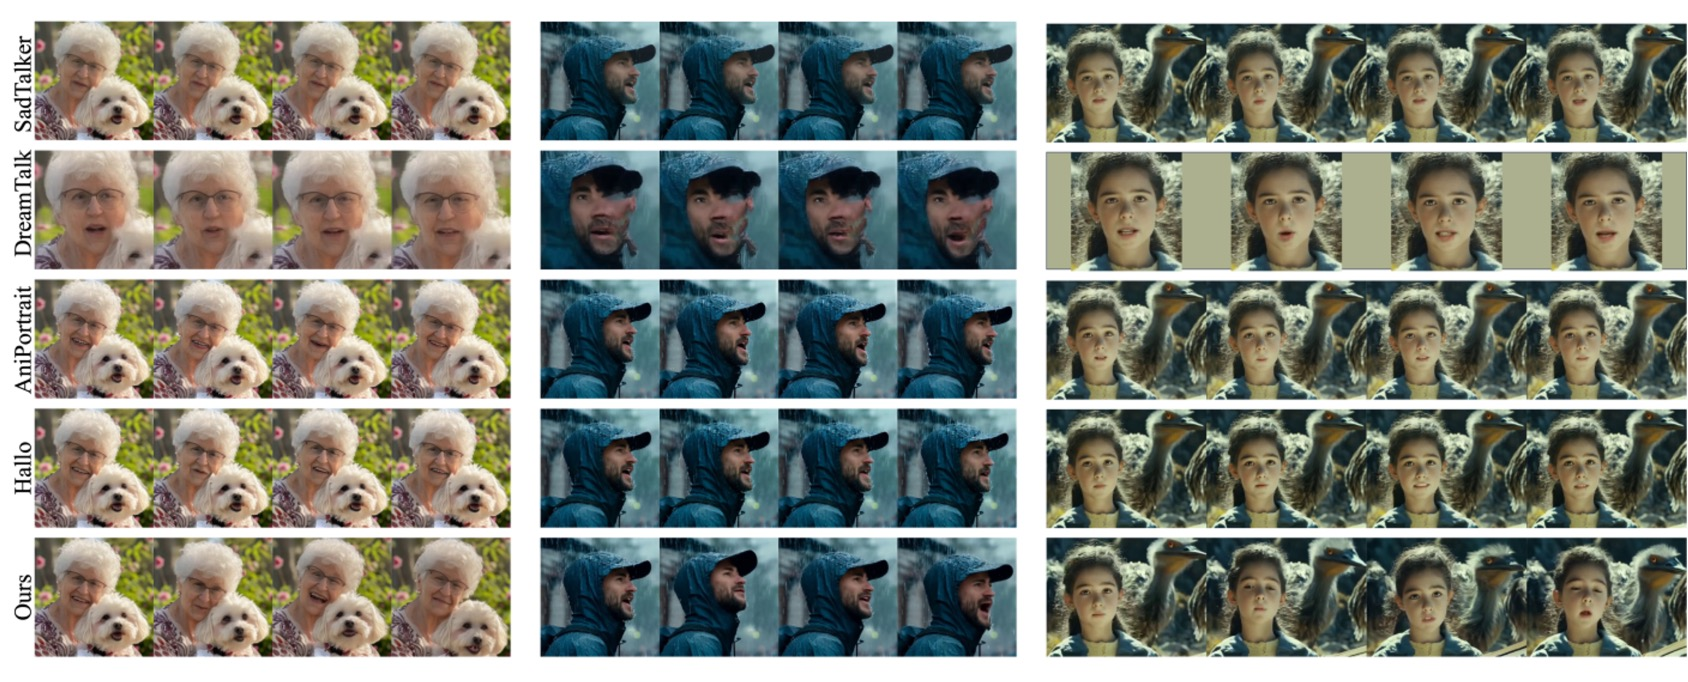
\includegraphics[width=1.01\linewidth]{figs/method_comparison3_2.jpg}
    \vspace{-7mm}
    \caption{Complex facial identity with dynamic accessories subjects and different pose orientation.}
    
    \label{fig:portrait_complex_face}
    \vspace{2mm}
\end{figure*}

\begin{figure*}[t!]
    \centering
    \includegraphics[width=1.0\linewidth]{figs/ComplexScenes.jpg}
    \vspace{-6mm}
    \caption{Complex scenes with dynamic foreground or background and various head poses.}
    \label{fig:ComplexScenes}
    \vspace{-2mm}
\end{figure*}










\subsection{Ablation Study and Discussion}
\label{sec:ablationstudy}
\noindent\textbf{Audio Conditioning.} {Table~\ref{tab:audio_injection} and Figure~\ref{fig:comparisn_of_audio_conditioning2} illustrate the effects of various strategies for incorporating audio conditioning. The results demonstrate that using cross-attention to integrate audio improves lip synchronization by enhancing the local alignment between visual and audio features, particularly around the lips. This is evident from the improvements in Sync-C and Sync-D, and it also contributes to a degree of enhancement in video quality.}

\noindent\textbf{Identity Reference Network.} {
Table~\ref{tab:identity_preserve} and Figure~\ref{fig:Comparison_of_the_appearance_reference_network} evaluate different identity conditioning strategies.  The results indicate that without an identity condition, the model fails to preserve the portrait appearance. When using face embedding alone, the model introduces blur and distortion, as it focuses solely on facial features and disrupts the global visual context. To address this, we introduce an identity reference network to preserve global features while making facial motion more controllable through identity-based facial embeddings. Thus, the proposed method achieves a lower FID of 23.458 and FVD of 242.602, while maintaining lip synchronization.
}

\noindent\textbf{Temporal Motion Frames.} {Table~\ref{tab:motion_frame_num} presents an analysis of varying temporal motion frames. One motion frame achieves the highest Sync-C score (6.889) and the lowest Sync-D score (8.695), indicating substantial lip synchronization.}

% \subsection{Limitations and Future Works}
% \textcolor{red}{This paper presents advancements in wild portrait image animation with different perspective and complex scenes, there exist several limitations that necessitate further exploration and consideration. (1)...}
% \begin{table}[]
% \centering
% \footnotesize
% \begin{tabular}{lc|l|l|l|l|l|l}
% \cline{2-8}
%  &
%   FD & PG &
%   \multicolumn{1}{c|}{FID$\downarrow$} &
%   \multicolumn{1}{c|}{FVD$\downarrow$} &
%   \multicolumn{1}{c|}{Sync-C$\uparrow$} &
%   \multicolumn{1}{c|}{Sync-D$\downarrow$} &
%   \multicolumn{1}{c}{E-FID$\downarrow$} \\ \cline{2-8} 
%  &            &            & - & - & - & - & - \\
%  & \checkmark &            & - & - & - & - & - \\
%  &            & \checkmark & - & - & - & - & - \\
%  & \checkmark & \checkmark & - & - & - & - & - \\ \cline{2-8} 
% \end{tabular}
% \caption{Ablation on augmentation for id preservation. FD: Frame drop; PG: Pixel Gaussian}
% \label{tab:abl_id_augment}
% \end{table}


\noindent
\textbf{CFG Scales for Diffusion Model.}  
Table~\ref{tab:abalation_cfg} provides a quantitative analysis of video generations using various CFG scales for audio, text, and reference images. A comparison between the second and fourth rows demonstrates that increasing the audio CFG scale enhances the model's ability to synchronize lip movements. The text CFG scale significantly influences the video’s dynamism, as indicated in the first three rows, where both the subject's and the background's dynamics increase with higher text CFG scales. Conversely, the reference image CFG scale primarily governs the subject's appearance; higher values improve subject consistency, as illustrated by the second and fifth rows. Among the tested configurations, setting \(\lambda_a=3.5\), \(\lambda_t=3.5\), and \(\lambda_i=1.0\) yields a balanced performance. This interplay between visual fidelity and dynamics underscores the effectiveness of CFG configurations in generating realistic portrait animations.


\begin{figure*}[!t]
    \centering
    \begin{minipage}{0.48\linewidth}
        \centering
        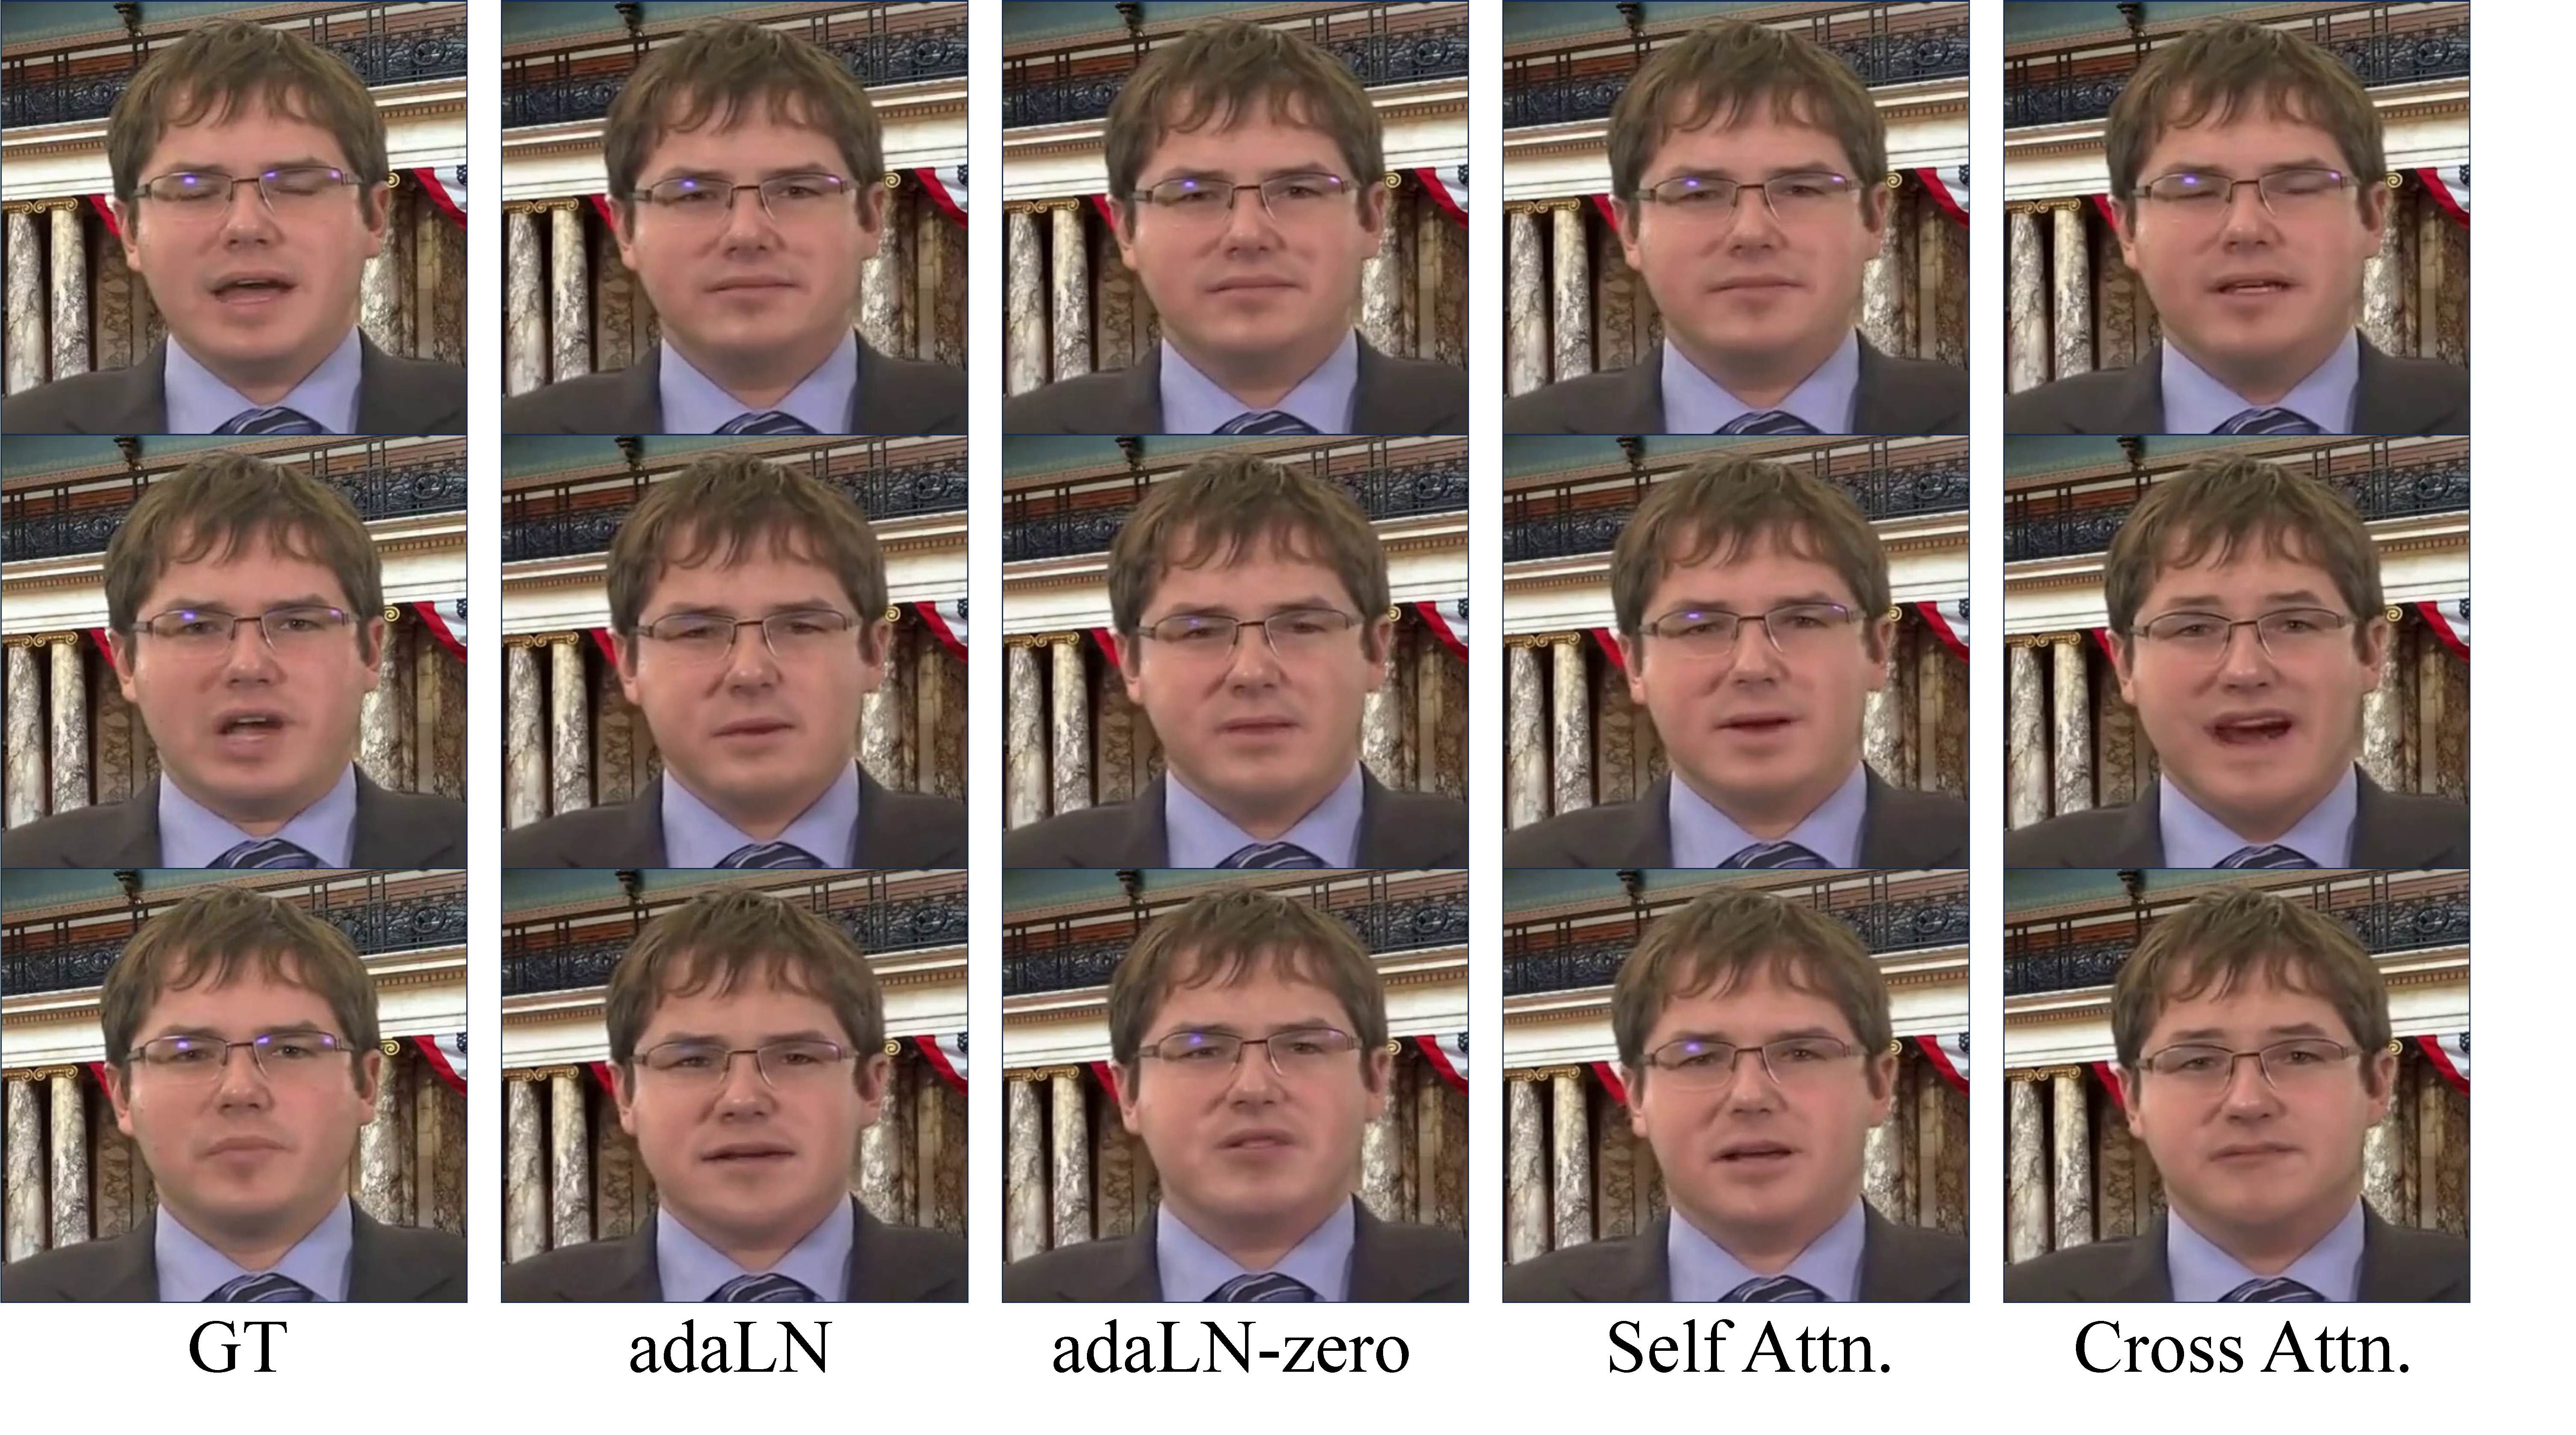
\includegraphics[width=\linewidth]{figs/comparisn_of_audio_conditioning3.pdf}
        \vspace{-7mm}
        \caption{Qualitative comparison of different strategies for audio conditioning.}
        \label{fig:comparisn_of_audio_conditioning2}
        \vspace{16.5mm}
    \end{minipage}
    \hfill% 手动添加间距
    \begin{minipage}{0.48\linewidth}
        \centering
        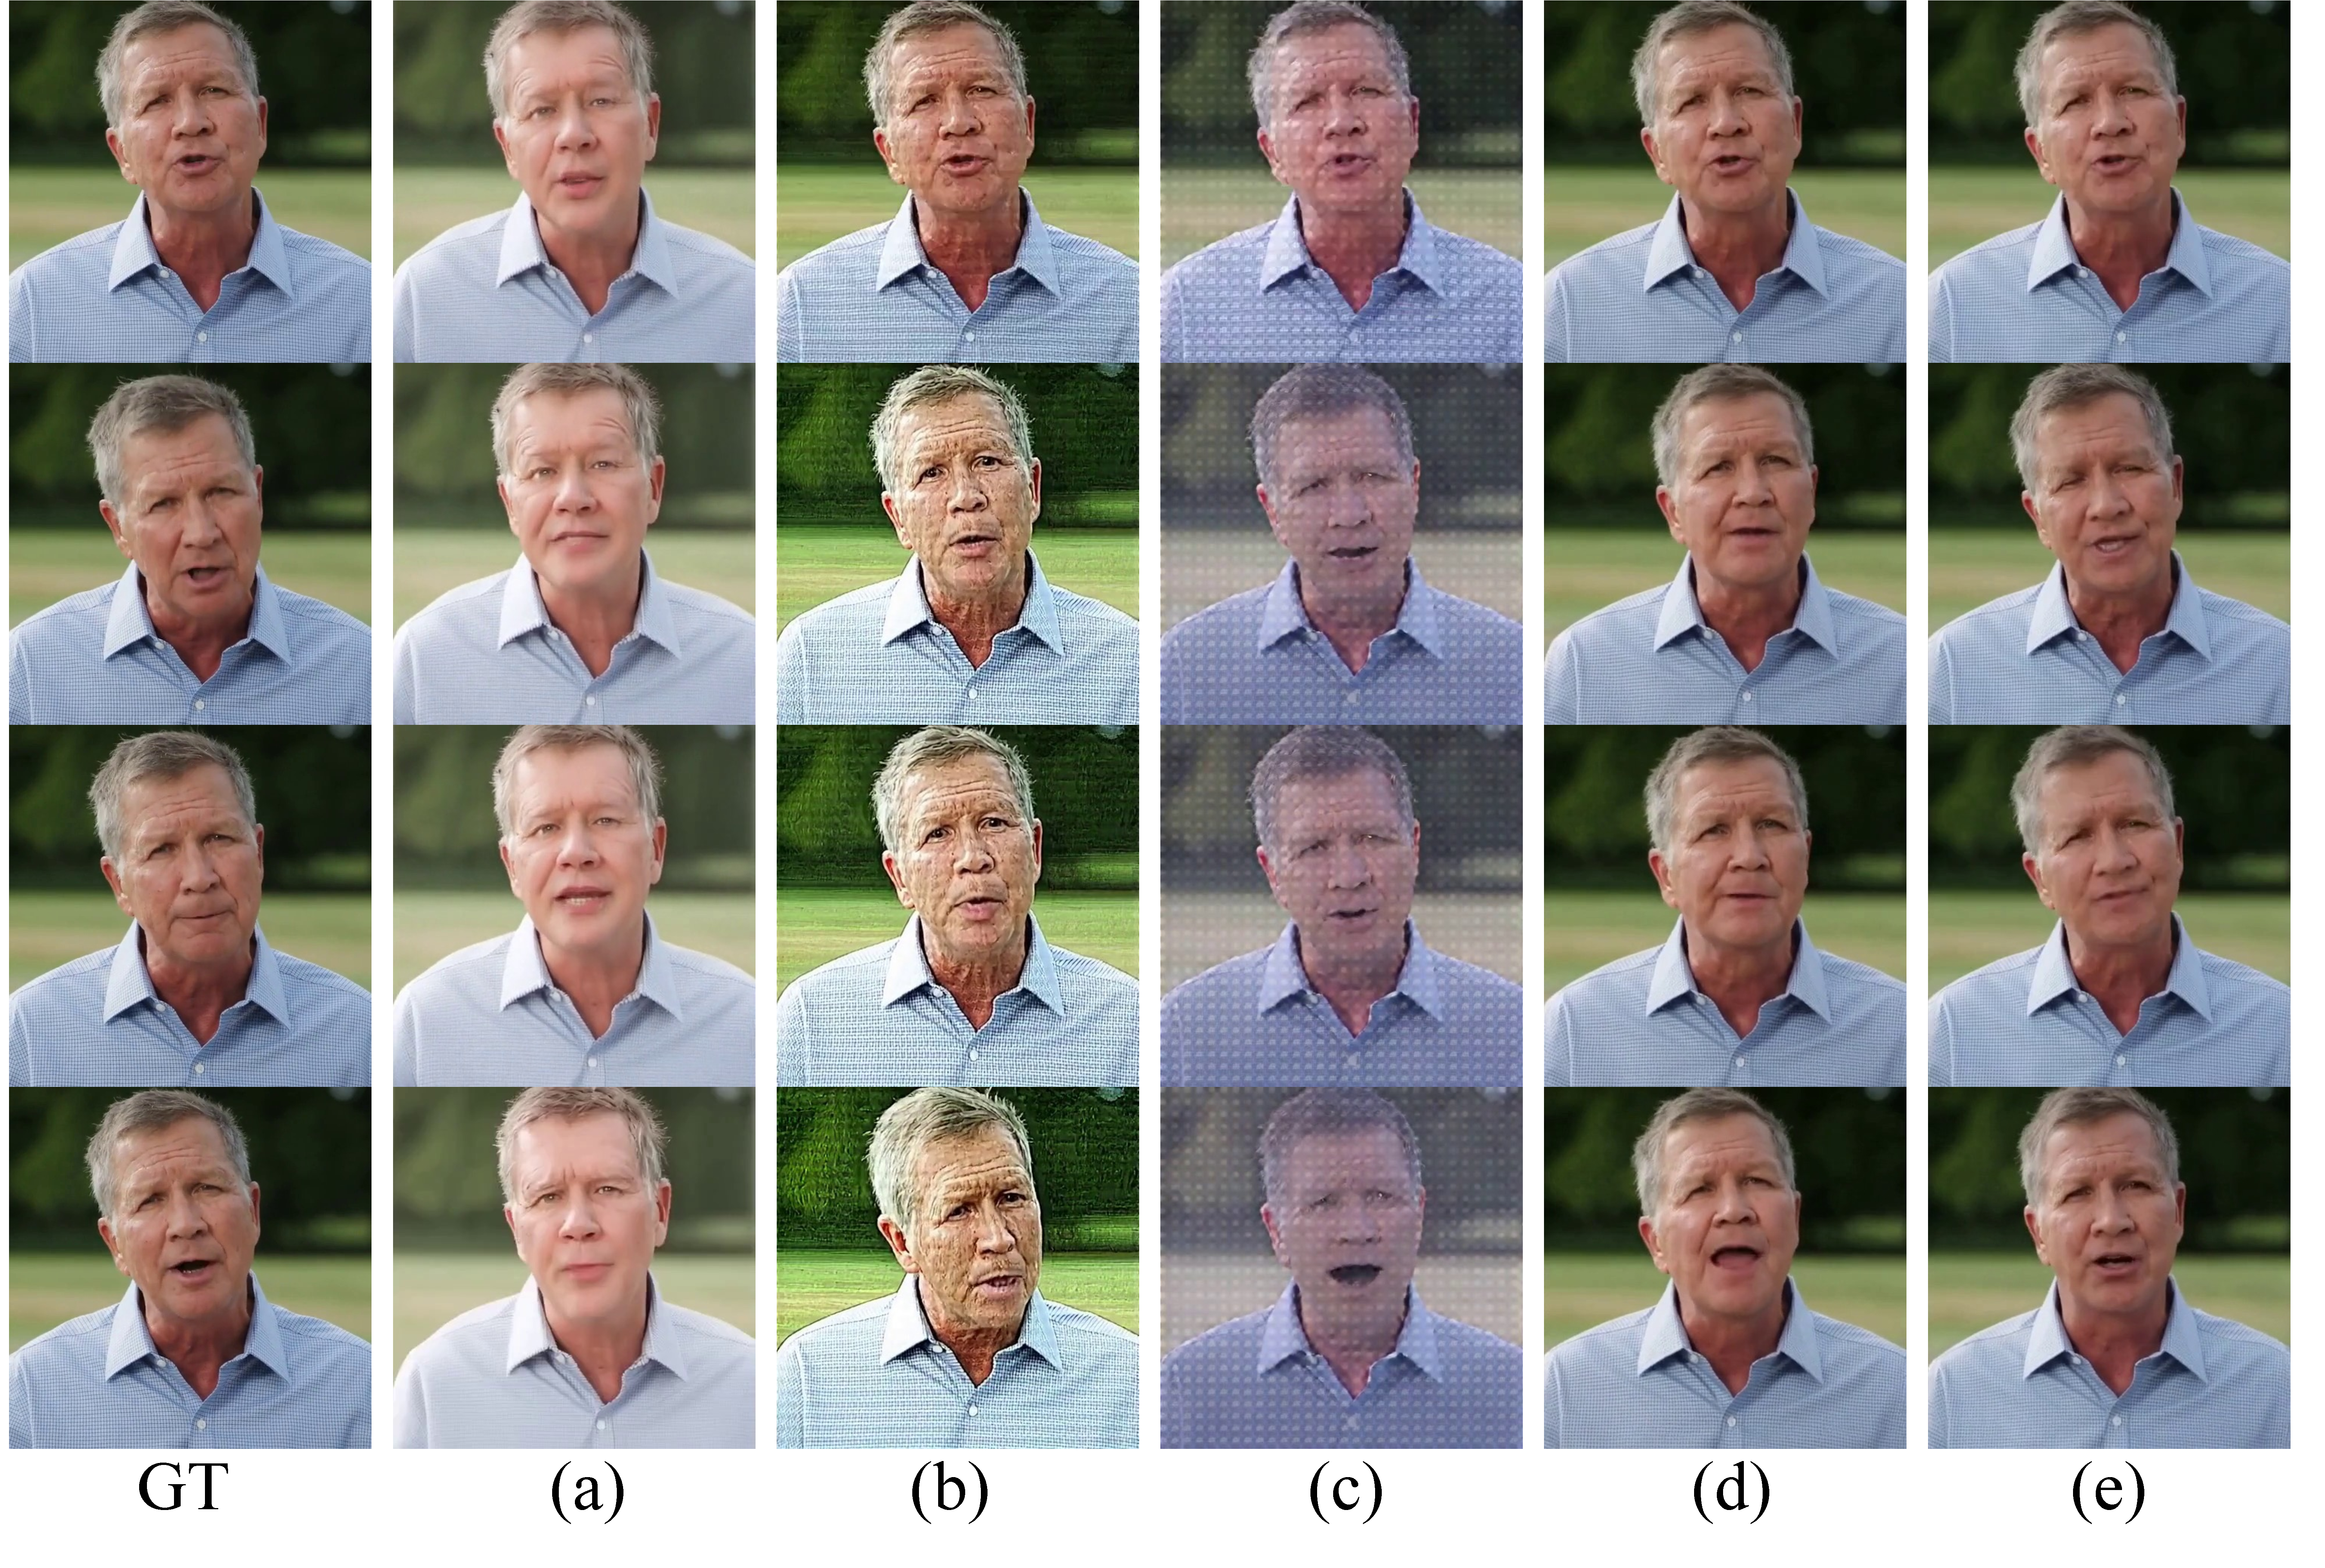
\includegraphics[width=1\linewidth]{figs/Comparison_of_the_appearance_reference_network2.pdf}
        \vspace{-7mm}
        \caption{Qualitative comparison of different strategies~(as in Table~\ref{tab:identity_preserve}) for identity conditioning. 
        (a) No identity condition; (b) Face attention; (c) Face adaptive norm; (d) Identity reference network; (e) Face attention and Identity reference network. 
        }
        \label{fig:Comparison_of_the_appearance_reference_network}
    \end{minipage}
    \vspace{-3mm}
\end{figure*}




\begin{table}[t!]
\vspace{-16mm}
\centering
\footnotesize
\resizebox{\linewidth}{!}{
\begin{tabular}{c|c|c|c|c}
\toprule
  \makecell{Audio Injection Method} &
  \multicolumn{1}{c|}{FID$\downarrow$} &
  \multicolumn{1}{c|}{FVD$\downarrow$} &
  \multicolumn{1}{c|}{Sync-C$\uparrow$} &
  \multicolumn{1}{c}{Sync-D$\downarrow$} \\ 
  \midrule
 adaLN       & 24.159 & 264.331 & 1.374 & 13.524 \\
 adaLN-zero  & 24.029 & 276.403 & 1.398 & 13.553 \\ 
 Self Attn.  & 24.748 & 270.101 & 1.345 & 13.456 \\
 \midrule
 Cross Attn.~(Ours) & \textbf{23.458} & \textbf{242.602} & \textbf{4.601} & \textbf{10.416} \\
 \bottomrule
\end{tabular}
}
\vspace{-2mm}
\caption{Comparison on the different strategy of audio conditioning.}
\label{tab:audio_injection}
\vspace{-1mm}
\end{table}


\begin{table}[t!]
\centering
\footnotesize
\resizebox{\linewidth}{!}{
\begin{tabular}{c|c|c|c|c|c}
\toprule
  \makecell{Identity Injection Method} &
  \multicolumn{1}{c|}{FID$\downarrow$} &
  \multicolumn{1}{c|}{FVD$\downarrow$} &
  \multicolumn{1}{c|}{Sync-C$\uparrow$} &
  \multicolumn{1}{c|}{Sync-D$\downarrow$} & 
  \multicolumn{1}{c}{ Subject Consistency$\uparrow$} \\ 
  \midrule
 (a) No identity condition & 32.304 & 371.820 & 3.183 & 11.732 & 0.977 \\
 (b) Face attention & 57.541 & 740.536 & 4.042 & 10.682 & 0.974 \\
 (c) Face adaptive norm & 150.720 & 1587.395 & 3.822 & 12.324 & 0.904 \\
 (d) Identity reference network & 28.789 & 291.863 & 4.553 & \textbf{10.317} & 0.984 \\
 \midrule
 (e) Face attention and Identity reference network  & \textbf{23.458} & \textbf{242.602} & \textbf{4.601} & 10.416 & \textbf{0.988} \\ 
 \bottomrule
\end{tabular}
}
\vspace{-2mm}
\caption{Comparison of different identity injection method. ``No identity condition'' refers to the absence of any conditioning related to identity; ``Face attention'' and ``Face adaptive norm'' involve incorporating face embeddings using self-attention and adaptive layer normalization, respectively. ``Identity reference network'' refers to the introduction of identity features using a reference network.}
\label{tab:identity_preserve}
\vspace{-1mm}
\end{table}

\begin{table}[t!]
\centering
\footnotesize
\resizebox{\linewidth}{!}{
\begin{tabular}{c|c|c|c|c}
\toprule
  \makecell{Motion Frame Number} &
  \multicolumn{1}{c|}{FID$\downarrow$} &
  \multicolumn{1}{c|}{FVD$\downarrow$} &
  \multicolumn{1}{c|}{Sync-C$\uparrow$} &
  \multicolumn{1}{c}{Sync-D$\downarrow$} \\ 
  \midrule 
 n = 1     & 24.040 & 242.708 & \textbf{6.889} & \textbf{8.695} \\
 n = 2     & \textbf{23.458} & \textbf{242.602} & 4.601 & 10.416 \\
 n = 4     & 24.459 & 269.904 & 5.109 & 10.489 \\
 n = 8     & 27.303 & 265.396 & 5.114 & 10.464 \\ 
 \bottomrule 
\end{tabular}
}
\vspace{-2mm}
\caption{Ablation on the number of motion frames.}
\label{tab:motion_frame_num}
\vspace{-6mm}
\end{table}

\begin{table*}[th!]
    \centering
    \resizebox{\linewidth}{!}{
    \begin{tabular}{c|ccc|c|c|c|c|c|c|c}
    \toprule
    &Audio & Text & Image & 
    Sync-C$\uparrow$ & Sync-D$\downarrow$ & 
    \makecell{Subject\\Dynamic$\uparrow$} & 
    \makecell{Background\\Dynamic$\uparrow$} & 
    \makecell{Subject\\FVD$\downarrow$} & 
    \makecell{Background\\FVD$\downarrow$} &
    \makecell{Subject\\Consistency$\uparrow$}\\ 
    \midrule
    $\lambda_t \downarrow$ &$\lambda_a = 3.5$ & $\lambda_t=1.0$ & $\lambda_i=1.0$ &  6.168 & 8.589 & 13.164 & \ \ \ 3.955 $\downarrow$ & 361.582 & 263.416 & 0.9813 \\ 
    Base &$\lambda_a=3.5$ & $\lambda_t=3.5$ & $\lambda_i=1.0$ &  6.154 & 8.574 & 13.286 & 4.481 & 359.493 & 248.283 & 0.9810 \\ 
    $\lambda_t \uparrow$ &$\lambda_a=3.5$ & $\lambda_t=6.0$ & $\lambda_i=1.0$ &  6.044 & 8.861 & 13.616 & \ \ \ 4.659 $\uparrow$ & 342.894 & 235.307 & 0.9808 \\ 
    $\lambda_a \uparrow$&$\lambda_a=6.0$ & $\lambda_t=3.5$ & $\lambda_i=1.0$ &  \ \ \ 6.469 $\uparrow$ & 8.515 & 14.778 & 4.066 & 379.073 & 264.969 & 0.9809 \\  
    $\lambda_i \uparrow$&$\lambda_a=3.5$ & $\lambda_t=3.5$ & $\lambda_i=3.5$ & 6.023 & 8.654 & 12.599 & 4.219 & 367.225 & 265.414 & \ \ \ 0.9835 $\uparrow$ \\ 
    \bottomrule
    \end{tabular}}
    \vspace{-3mm}
    \caption{ Quantitative study of audio, text and image CFG scales on our proposed wild dataset. }
    \vspace{-2mm}
    \label{tab:abalation_cfg}
\end{table*}

\noindent\textbf{Limitations and Future Works.}
Despite the advancements in portrait image animation techniques presented in this study, several limitations warrant acknowledgment. 
While the proposed methods improve identity preservation and lip synchronization, the model's ability to realistically represent intricate facial expressions in dynamic environments still requires refinement, especially under varying illumination conditions. 
Future work will focus on enhancing the model's robustness to diverse perspectives and interactions, incorporating more comprehensive datasets that include varied backgrounds and facial accessories. 
Furthermore, investigating the integration of real-time feedback mechanisms could significantly enhance the interactivity and realism of portrait animations, paving the way for broader applications in live media and augmented reality.

\noindent\textbf{Safety Considerations.}
The advancement of portrait image animation technologies, particularly those driven by audio inputs, presents several social risks, most notably concerning the ethical implications associated with the creation of highly realistic portraits that may be misused for deepfake purposes. 
To address these concerns, it is essential to develop comprehensive ethical guidelines and responsible use practices.
Moreover, issues surrounding privacy and consent are prominent when utilizing individuals' images and voices. It is imperative to establish transparent data usage policies, ensuring that individuals provide informed consent and that their privacy rights are fully protected.
By acknowledging these risks and implementing appropriate mitigation strategies, this research aims to promote the responsible and ethical development of portrait image animation technology.

\subsection{Generation Controllability}

\noindent\textbf{Textual Prompt for Subject Animation.}
To evaluate whether textual conditional controllability is effectively preserved, we conducted a series of experiments comparing the performance of our method to that of the baseline model, CogVideoX~\cite{yang2024cogvideox}, using same text prompts. As shown in Figure~\ref{fig:inter}, the results shows that our model maintains its ability for textual control, and effectively captures the interaction between different subjects as dictated by the textual prompts.
% (e.g.,the rabbit, horse and birds.)

\noindent\textbf{Textual Prompt for Foreground and Background Animation.} We also explore model's ability to follow the foreground and background textual prompt. As illustrated in Figure~\ref{fig:fgbg}, our method animates the foreground and background subjects naturally, such as the ocean waves and flickering candlelight. The results demonstrates the model's ability to control foreground, and background with the textual caption, which is maintained even after introducing the audio condition.

\begin{figure*}[!h]
    \centering
    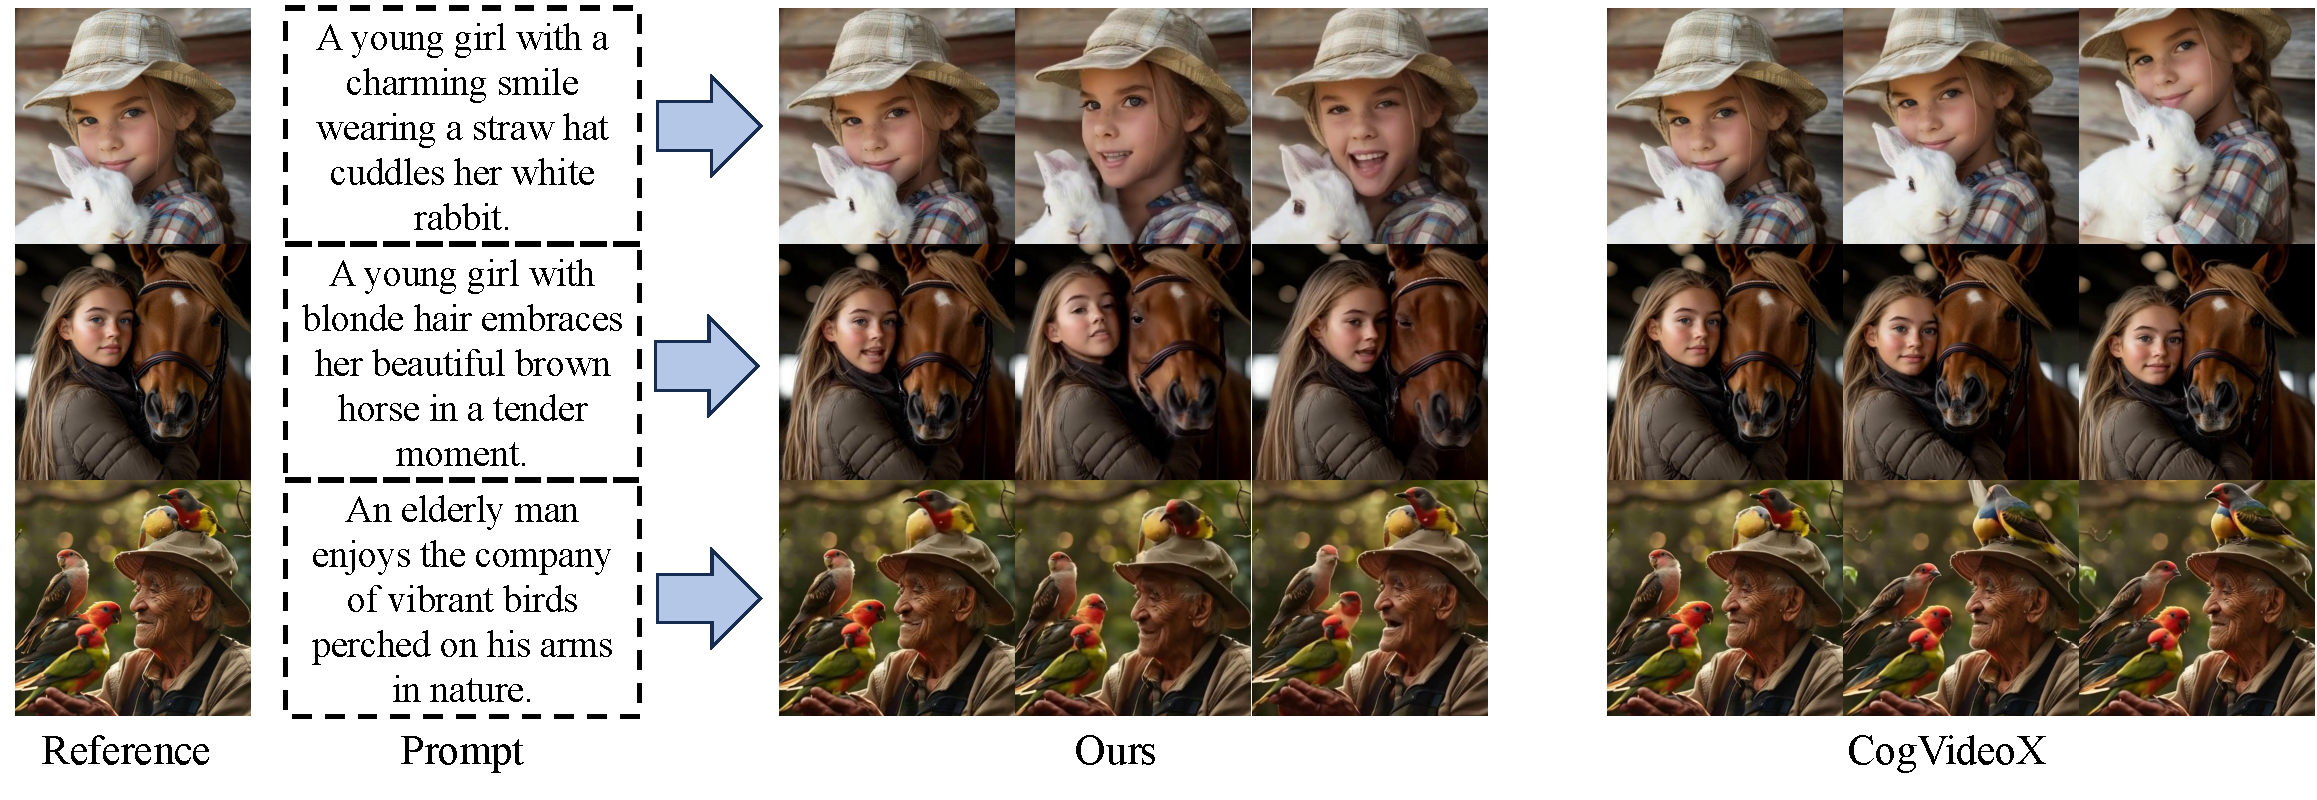
\includegraphics[width=.97\linewidth]{figs/text_cond_interact.pdf}
    \vspace{-4mm}
    \caption{{Condition on interacting with subjects. Our method achieves alignment comparable to that of CogVideX, maintaining the controllability of interactive subjects even after introducing the audio condition.}}
    \vspace{-2mm}
    \label{fig:inter}
\end{figure*}

\begin{figure*}[!h]
    \centering
    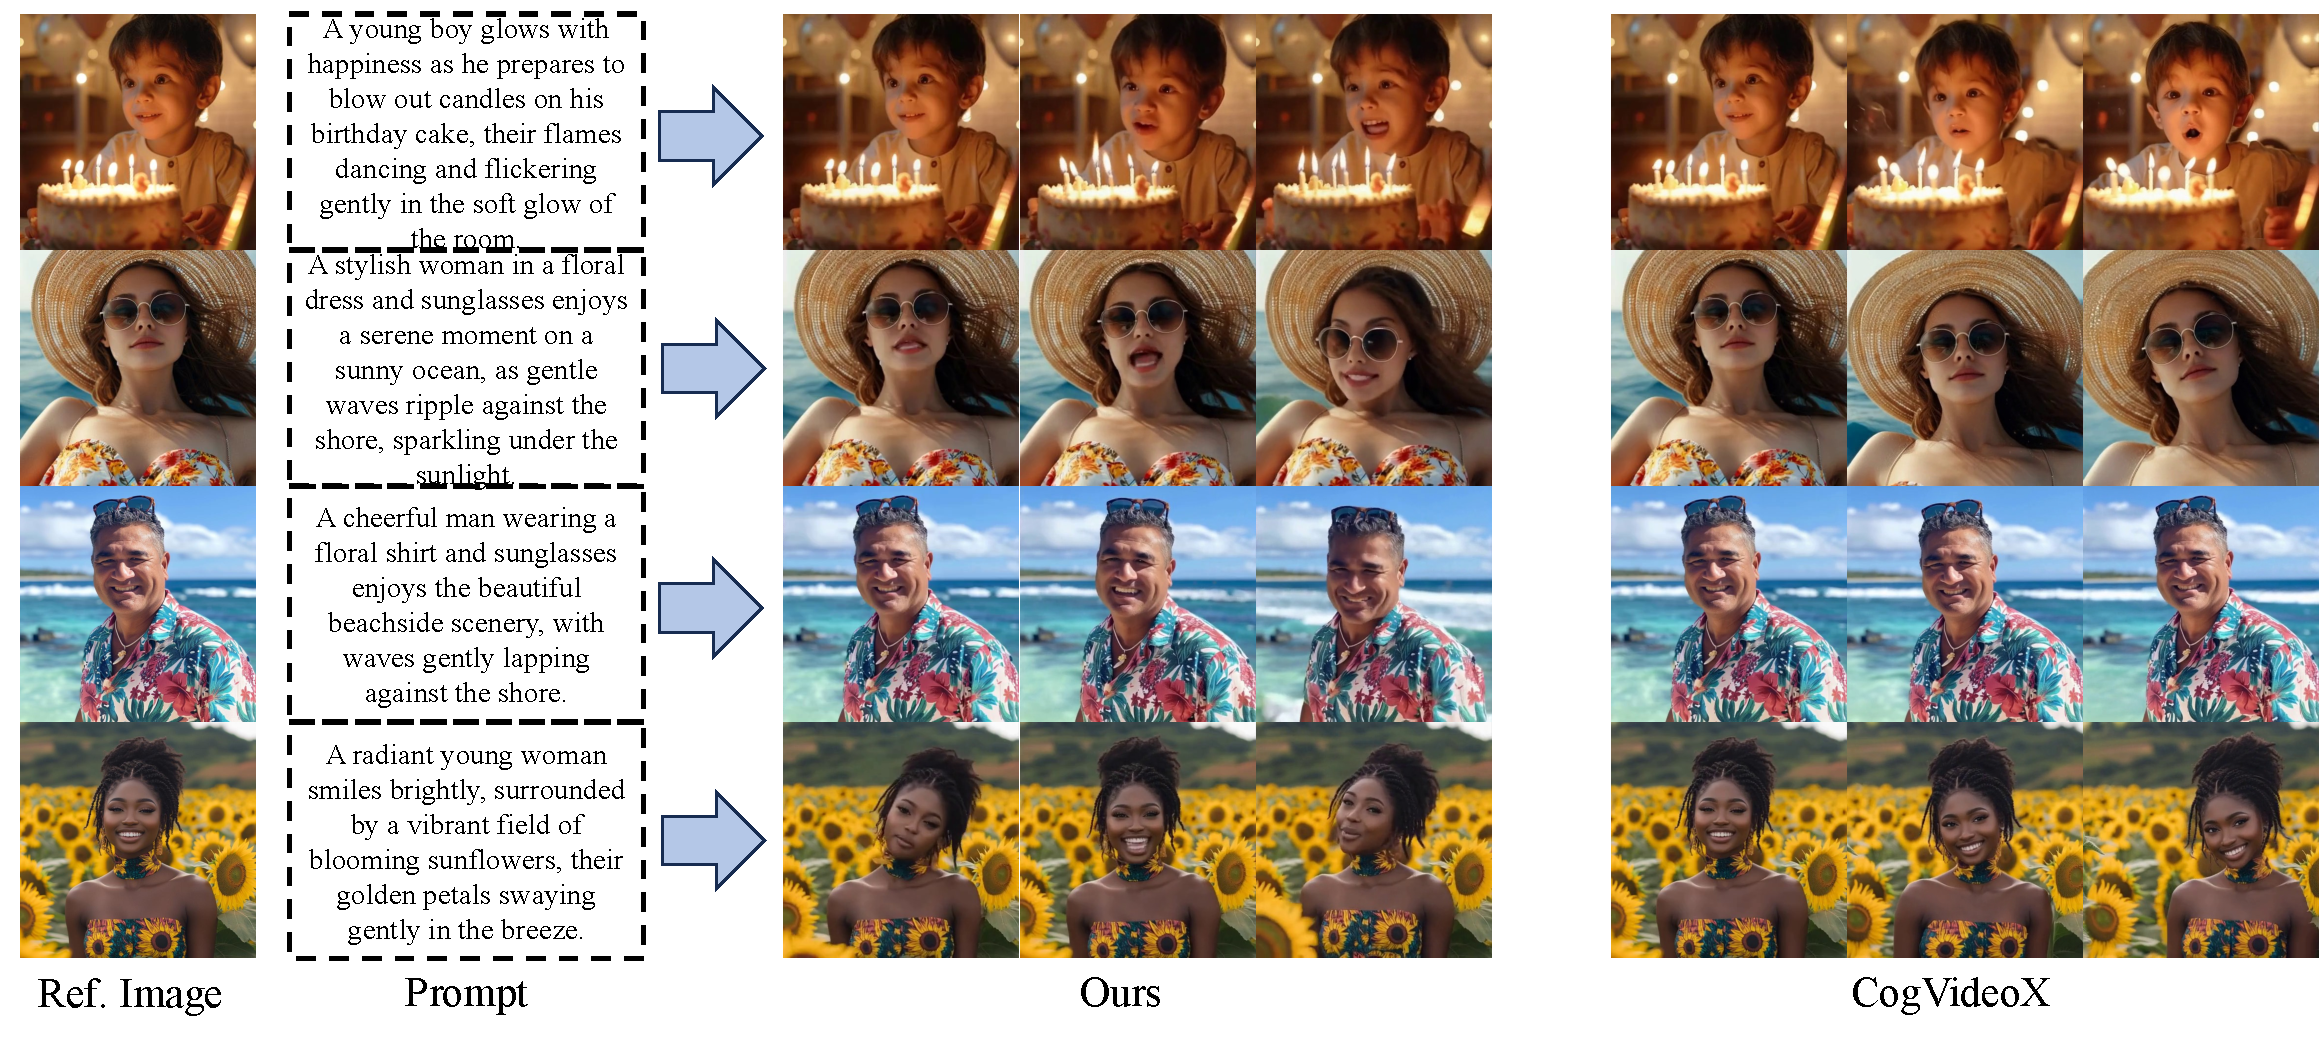
\includegraphics[width=.97\linewidth]{figs/text_cond_bgfg.pdf}
    \vspace{-4mm}
    \caption{{Textual condition on foreground and background. Our method achieves alignment comparable to that of CogVideX, maintaining the controllability of foreground and background after incorporating the audio condition. }}
    \label{fig:fgbg}
    \vspace{-3mm}
\end{figure*}
